\section{Нейронные сети в Computer Vision}
\begin{center}
    Конспект составил: \textit{Никита Немакин}
\end{center}

\subsection{Математическая модель нейрона}

Для моделирования нейронных сетей с помощью компьютеров была создана сильно упрощённая математическая модель нейрона (рис. \ref{neuron}).

\begin{figure}[H]
    \centering
    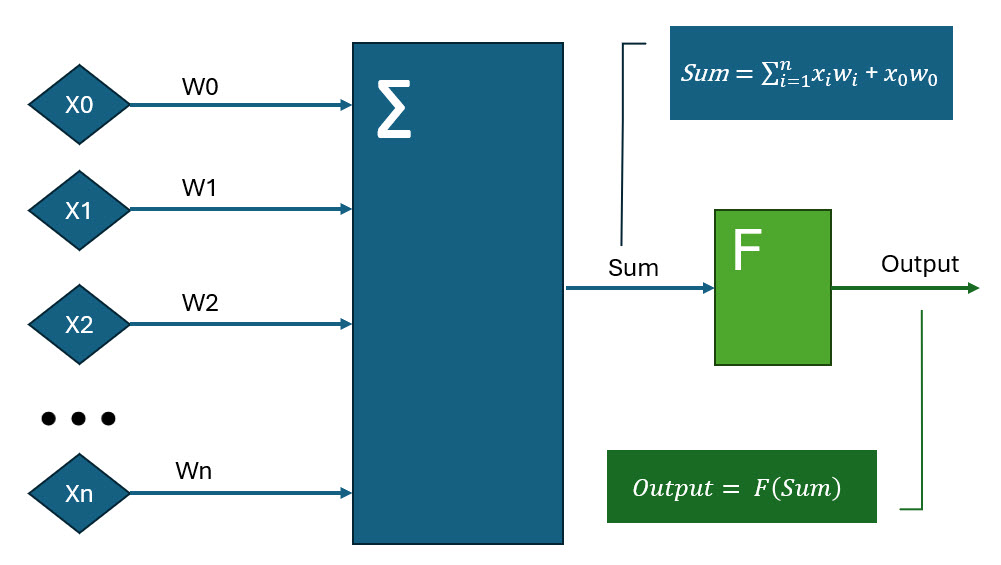
\includegraphics[width = 12cm]{neuron.jpg}
    \caption{Математическая модель нейрона}
    \label{neuron}
\end{figure}

Здесь входные сигналы $X_0,…,X_n$ попадают на вход взвешенного сумматора, при этом веса $W_0,…,W_n$ определяют «вклад» каждого сигнала на итоговую сумму $Sum$. Этот вклад может быть положительным или отрицательным, увеличивающим или уменьшающим значение суммы. Сигнал $X_0$ и соответствующий ему вес $W_0$ может использоваться для инициализации нейрона.

Результат вычисления взвешенной суммы попадает на вход передаточной функции $F$ (функцией активации). Эта функция определяет зависимость выходного сигнала нейрона от взвешенной суммы сигналов на его входах. Обычно активация наступает при превышении определенного порога.

На практике применяются линейные и сигмоидные функции, функции гиперболического тангенса, функции Rectified Linear Unit (выпрямленный линейный блок), Leaky ReLU и другие (рис. \ref{funcs})

\begin{figure}[H]
    \centering
    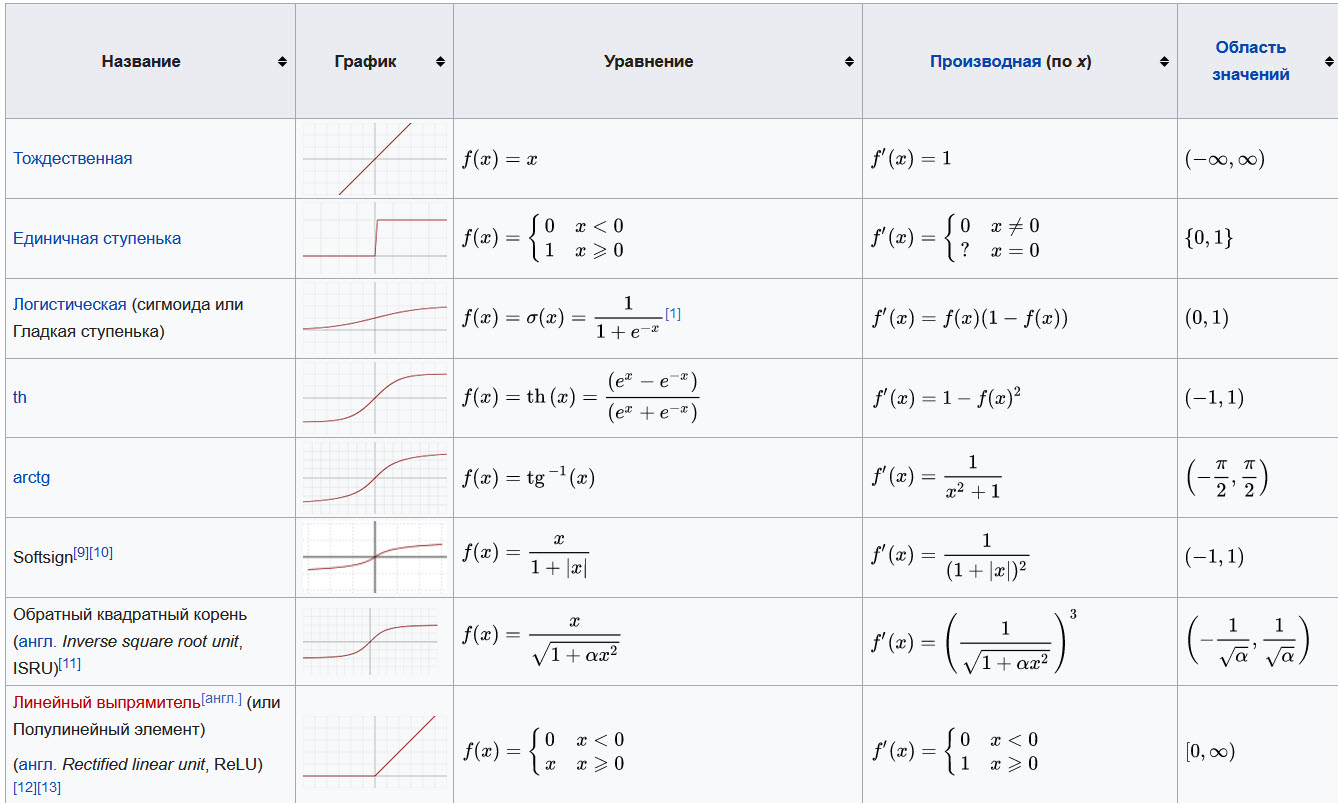
\includegraphics[width = 12cm]{funcs.jpg}
    \caption{Некоторые из функций активации}
    \label{funcs}
\end{figure}

Какую из функций следует использовать? Тут нет однозначного ответа. Функция активации влияет на скорость обучения и работы сети. Она может подбираться в процессе экспериментов или исследований. Когда мы имеем дело с готовыми моделями нейросетей и фреймворками, нам не придётся выбирать функцию активации самостоятельно.

\subsection{Архитектуры нейронных сетей}

\subsubsection*{Перцептрон}
Нейроны можно комбинировать в нейронную сеть, пригодную, например, для распознавания простейших изображений.\\

На рис. \ref{perceptron} показан так называемый перцептрон — простейший вид нейронной сети, состоящей из входного и выходного слоев. В примере он используется для распознавания цифр в диапазоне от 0 до 9.

\begin{figure}[H]
    \centering
    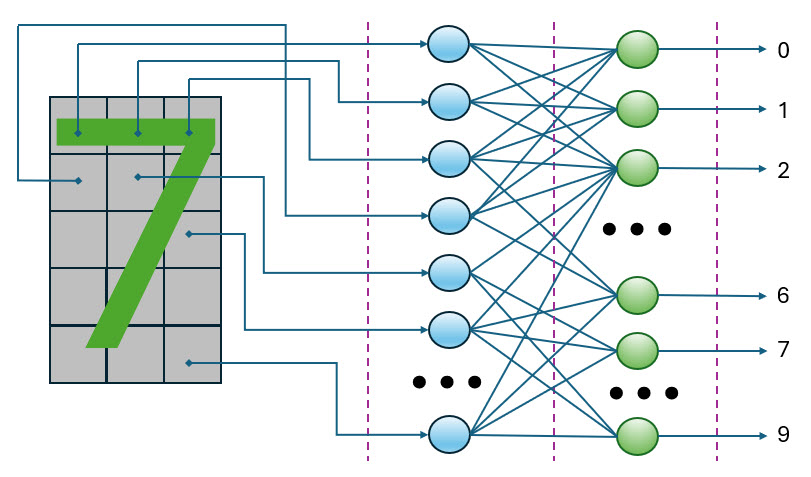
\includegraphics[width = 12cm]{perceptron.jpg}
    \caption{Использование перцептрона для распознавания цифр}
    \label{perceptron}
\end{figure}

В левой части рисунка показана матрица, в узлах которой находятся фотоэлементы или аналогичные устройства. Эти устройства способны посылать в нейроны входного слоя сигналы 0 или 1 в зависимости от того, перекрыт фотоэлемент изображением цифры или нет.

Выходы нейронов первого слоя соединены со входами второго, выходного слоя нейронов. Хотя на рис. \ref{perceptron} это и не показано, предполагается, что каждый выход нейрона входного слоя соединен со входами всех нейронов выходного слоя.

Выходной слой содержит ровно десять нейронов, по одному на каждую цифру.

В процессе обучения сети предъявляются разные цифры и настраиваются веса для нейронов выходного слоя таким образом, чтобы активировался только тот нейрон, который соответствует предъявленной цифре. Заметим, что входной слой нейронов предназначен только для передачи сигналов от фотоэлементов на нейроны выходного слоя, и его веса в процессе обучения не изменяются.

Для обучения данной сети используется так называемый метод коррекции ошибки:
\begin{itemize}
    \item На первом шаге с помощью генератора случайных чисел всем весам присваиваются небольшие значения.
    \item Далее перцептрону предъявляется одна из цифр, после чего для каждого нейрона вычисляется его ошибка.
    \item Затем производится корректировка весов, и ошибка вычисляется снова.
\end{itemize}

Вся эта процедура повторяется необходимое количество раз до тех пор, пока ошибка не исчезнет. Подобное обучение нужно будет провести для каждой цифры, на что может уйти довольно много времени.

\subsubsection*{Сверточные сети}

Перцептрон плохо подходит для распознавания объектов на изображениях в реальном времени, не говоря уж о кадрах видеопотока.

Например, если размер изображения составляет 640x480 пикселей, то во входной нейронной сети, подобной описанной выше, нужно будет использовать 307200 нейронов. В процессе распознавания по обученной сети, содержащей сотни тысяч нейронов и сотни миллионов связей, придётся делать очень много вычислений.

Наша цель — организовать обнаружение объектов, для которых обучение не выполнялось, причем в реальном времени. Например, обнаружить и выделить на фотографии или в видеопотоке лица или фигуры людей (или других объектов), которые нейронная сеть никогда не «видела».

Перцептрон с этой задачей не справится из-за своих ограничений. Но главное — перцептрон не учитывает особенности изображений, в частности, взаимное расположение частей изображения. Перцептрон работает с векторами, и в нем нет ничего специального для поиска объектов на изображениях.\\

Для решения задач компьютерного зрения, классификации и сегментации изображений, а также для обнаружения объектов были созданы так называемые сверточные нейронные сети (Convolutional Neural Network, CNN).

Сверточные сети учитывают двумерную топологию изображений. Они устойчивы к небольшим смещениям, изменениям масштаба и поворотам объектов на входных изображениях.\\

\begin{figure}[H]
    \centering
    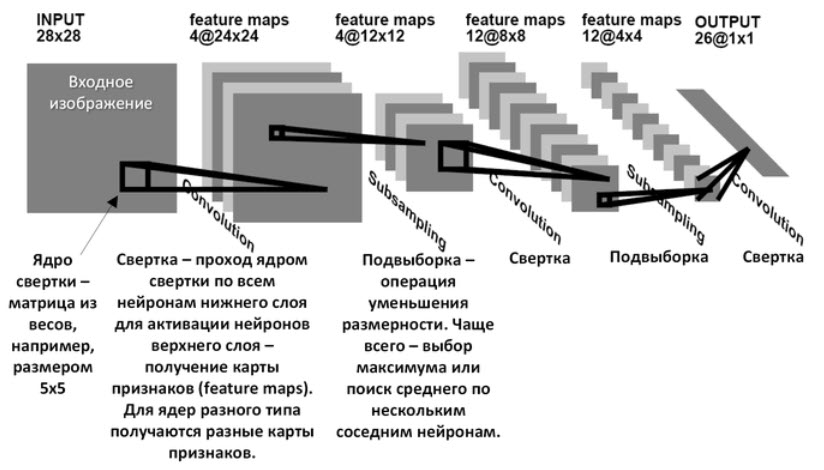
\includegraphics[width = 12cm]{cnn.jpg}
    \caption{Архитектура сверточной нейронной сети}
    \label{cnn}
\end{figure}

Можно выделить следующие компоненты сверточной нейронной сети:
\begin{itemize}
    \item сверточные слои (Convolutional Layers);
    \item слои подвыборки (Pooling Layers);
    \item слой активации;
    \item полносвязные слои (Fully Connected Layers);
\end{itemize}

Сверточные слои позволяют нейронной сети «понимать» изображения, выделяя на них важные особенности, такие как грани, текстуры или формы объектов. Свертка позволяет обнаруживать различные уровни абстракции — низкоуровневые, такие как края и текстуры, и более высокоуровневые, такие как формы и объекты.

Слои подвыборки уменьшают размерность пространства признаков, уплотняя их представление и извлекая наиболее значимые признаки из каждой области. Это помогает улучшить распознавание при изменении масштаба изображения, а также при сдвигах объектов на изображении.

Слой активации играет роль функции активации, которая применяется к каждому числу входного изображения (рис. \ref{funcs}). Слой активации может быть встроен в сверточный слой и не показан на рис. \ref{cnn}.

Полносвязные слои содержат матрицы весовых коэффициентов и векторы смещений. Они используются для классификации или регрессии.

Сверточная сеть обучается с помощью алгоритма обратного распространения ошибки. Сначала выполняется прямое распространение от первого слоя к последнему, после чего вычисляется ошибка на выходном слое и распространяется обратно. При этом на каждом слое вычисляются градиенты обучаемых параметров, которые в конце обратного распространения используются для обновления весов с помощью градиентного спуска.

Операция обучения сверточной сети, как и перцептрона, длительная и достаточно ресурсоемкая.

\subsubsection*{Алгоритм обнаружения объектов YOLO}

Алгоритм YOLO (You Only Look Once) представляет собой чрезвычайно быстрый алгоритм обнаружения объектов, использующий сверточную нейронную сеть, и способный работать в режиме реального времени.

При использовании YOLO для ускорения обнаружения объектов предлагается выбрать в изображении некоторое фиксированное количество прямоугольников и для каждого прямоугольника проверить наличие искомого объекта. Если объект найден, для него определяется класс принадлежности и координаты рамки, окружающей этот объект — bounding box.

Класс принадлежности объекта — это такие категории, как «автомобиль», «дом», «пешеход», «стол», «машина», «грузовик», «автобус» и так далее.

Для каждого обнаруженного объекта YOLO возвращает рамку, окружающую этот объект (bounding box), а также вероятность принадлежности к тому или иному классу.

В отличие от традиционных сверточных сетей, YOLO способна обнаружить объекты за один проход по изображению, вместо множества таких проходов. Это существенно уменьшает время работы алгоритма. Во время этого единственного прохода с помощью сверточных слоев из изображения извлекаются признаки. В результате нет необходимости многократного выполнения свертки и пулинга.

Далее, YOLO разбивает изображение на сетку ячеек и предсказывает объекты, находящиеся в каждой ячейке. В результате алгоритм может эффективно обрабатывать изображения большого размера.

Архитектура YOLO позволяет задействовать мощности графических процессоров GPU. Это дает дополнительную прибавку скорости при работе сети на компьютерах, оснащенных такими процессорами.

\subsection{Распознавание образов}

Распознавание образов — важная задача CV, используемая для обнаружения экземпляров визуальных объектов определенных классов (например, людей, животных, автомобилей и зданий) в цифровых изображениях.
Где используется распознавание образов:

\paragraph{Лица людей}
Большинство систем распознавания лиц основаны на распознавании объектов. Его можно использовать для обнаружения лиц, классификации эмоций или выражений и подачи полученного поля в систему поиска изображений для идентификации конкретного человека из группы.
Обнаружение людей также обычно используется для подсчета количества людей в розничных магазинах или обеспечения показателей социального дистанцирования.

\paragraph{Интеллектуальная видеоаналитика} Обнаружение объектов используется в интеллектуальной видеоаналитике (IVA) везде, где в торговых точках присутствуют камеры видеонаблюдения, чтобы понять, как покупатели взаимодействуют с продуктами. Эти видеопотоки проходят через конвейер анонимизации, чтобы размыть лица людей и обезличить их. Некоторые варианты использования IVA сохраняют конфиденциальность, глядя только на обувь людей, размещая камеры ниже уровня колен и гарантируя, что система фиксирует присутствие человека, без необходимости непосредственно смотреть на его идентифицируемые черты. IVA часто используется на заводах, в аэропортах и транспортных узлах для отслеживания длины очередей и доступа в зоны ограниченного доступа.

\paragraph{Автономные транспортные средства}
Беспилотные автомобили используют обнаружение объектов, чтобы обнаруживать пешеходов, другие автомобили и препятствия на дороге, чтобы безопасно передвигаться. Автономные транспортные средства, оснащенные LIDAR, иногда используют 3D-обнаружение объектов, при котором вокруг объектов применяются прямоугольные формы.

\paragraph{Интеллектуальная видео хирургия}
Хирургическое видео — это очень зашумленные данные, которые снимаются с эндоскопов во время ответственных операций. Обнаружение объектов можно использовать для обнаружения трудно различимых объектов, таких как полипы или поражения, которые требуют немедленного вмешательства хирурга. Он также используется для информирования персонала больницы о статусе операции.

\paragraph{Проверка дефектов}
Компании-производители могут использовать обнаружение объектов для выявления дефектов на производственной линии. Нейронные сети можно научить обнаруживать мельчайшие дефекты, от складок на ткани до вмятин или вспышек в литьевых пластмассах.

В отличие от традиционных подходов к машинному обучению, обнаружение объектов на основе глубокого обучения также может обнаруживать дефекты в сильно различающихся объектах, таких как продукты питания.

\paragraph{Обнаружение пешеходов}
Это одна из важнейших задач компьютерного зрения, которая применяется в робототехнике, видеонаблюдении и автомобильной безопасности. Обнаружение пешеходов играет ключевую роль в исследованиях обнаружения объектов, поскольку оно предоставляет фундаментальную информацию для семантического понимания видеоматериалов.

\paragraph{AI-навигация дрона}
В наши дни дроны могут использовать модели, размещенные в облаке, для оценки любого объекта, с которым они сталкиваются.

Например, их можно использовать для осмотра труднодоступных участков мостов на наличие трещин и других структурных повреждений или для осмотра линий электропередач, заменяя опасные рутинные вертолетные операции.